%   % !TEX root = ../../VIII,3_Rahmen-TeX_8-1.tex
%
%
%   Band VIII, 3 N.~??S01.06
%   Signatur/Tex-Datei: LH_35_09_23_011-012
%   RK-Nr. 41208 /6
%   Überschrift: De corporum concursus scheda quinta
%   Modul: Mechanik / Stoß ( )
%   Datierung: Januar 1678
%   WZ: LEd-WZ 803003 = RK-WZ 142 (eins)
%   SZ: \groesser; \kleiner (insgesamt zwei)
%   Bilddateien (PDF): LH_35_09_23_011-012_d (insgesamt: eine)
%   Verzeichniseinträge: vollständig
%   \textls{} statt \textso{} (Ausnahme: Personenverzeichnis)
%
%
\selectlanguage{ngerman}%
\frenchspacing%
%
\begin{ledgroupsized}[r]{120mm}%
\footnotesize%
\pstart%
\noindent\textbf{Überlieferung:}%
\pend%
\end{ledgroupsized}%
\begin{ledgroupsized}[r]{114mm}%
\footnotesize%
\pstart%
\parindent -6mm%
\makebox[6mm][l]{\textit{L}}%
Konzept: LH~XXXV~9,~23 Bl.~11\textendash12.
Ein Bogen 2\textsuperscript{o};
ein Wasserzeichen auf Bl.~11;
Ausfransung mit geringfügigem Textverlust am Rand von Bl.~11~r\textsuperscript{o}.
Vier vollbeschriebene Seiten,
die den Text N.~\ref{dcc_04} %??S01\textsubscript{5} 
fortsetzen und vom Text N.~\ref{dcc_06-1} %??S01\textsubscript{7} 
fortgesetzt werden;
ein Kustos am Ende von Bl.~12~v\textsuperscript{o} verweist auf die \textit{Scheda sexta}.
% ??? Einige Randbemerkungen sind von Leibniz erst \textit{post reformationem} hinzugefügt worden (siehe die Vorbemerkung, S.~\refpassage{dcc_Vorbemerkung_reform-1}{dcc_Vorbemerkung_reform-2}).
\pend%
\end{ledgroupsized}%
%
\begin{ledgroupsized}[r]{114mm}%
\footnotesize%
\pstart%
\parindent -6mm%
\makebox[6mm][l]{\textit{E}}%
\textsc{Fichant} 1994, S.~106\textendash115\cite{01056}
(mit kommentierter französischer Übersetzung, S. 229\textendash236).
\pend%
\end{ledgroupsized}%
%
\selectlanguage{latin}%
\frenchspacing%
%
%
\vspace{8mm}
\count\Bfootins=1000%
\count\Afootins=1200%
\count\Cfootins=1000%%
\normalsize%
\pstart%
\noindent%
%
\lbrack11~r\textsuperscript{o}\rbrack% \ %  %  %  %  Blatt 11r
%
\hspace{47mm}
Scheda quinta%
\protect\index{Sachverzeichnis}{scheda}%
\hspace{36mm}
Januar. 1678%
\pend%
\pstart%
\noindent%
\centering%
De concursu
\edlabel{LH_35_09_23_011-012_11r1}%
corporum%
\protect\index{Sachverzeichnis}{concursus corporum}
\pend%
\vspace{0.5em}%
%
\pstart%
\noindent%
\edtext{}{%
{\xxref{LH_35_09_23_011-012_11r1}{LH_35_09_23_011-012_11r2}}%
{\lemma{corporum}\Bfootnote{%
\textit{(1)}~Hactenus absolvi
\textit{(2)}~Superest%
~\textit{L}}}}%
%
\edlabel{LH_35_09_23_011-012_11r2}%
\edtext{Superest
ut calculo comprehendam casum,%
\protect\index{Sachverzeichnis}{casus duplex}
quo corpus incurrit in aliud majus,%
\protect\index{Sachverzeichnis}{corpus minus in majus}
duplicem scilicet,
unum cum repellitur,%
\protect\index{Sachverzeichnis}{casus repulsae}
alterum cum progreditur.%
\protect\index{Sachverzeichnis}{casus progressus}%
}{%
\lemma{\textit{Am Rand:}}\Afootnote{%
Hic calculus nullius momenti.%
\protect\index{Sachverzeichnis}{calculus nullius momenti}%
\textsuperscript{\lbrack a\rbrack}%
{\footnotesize%
\newline\vspace{-0.4em}%
\newline%
\textsuperscript{\lbrack a\rbrack}~%
nullius momenti:
Die Rechnung beruht auf hinfälligen Annahmen und ist zudem fehlerhaft.%
\newline%
}}}
%
Incipiamus a casu progressus:%
\protect\index{Sachverzeichnis}{casus progressus}
\pend%
%
\pstart%
\noindent%
\edtext{}{%
{\xxref{LH_35_09_23_011r_ersteMarg_ytv-1}{LH_35_09_23_011r_ersteMarg_ytv-2}}%
{\lemma{\textit{Am Rand:}}\Afootnote{%
Si $A \,\sqcap\, 1$
et \textit{B} aequ. 2,
et $A \protect\underset{\displaystyle \textit{(B)}}{\textit{(A)}}$
aequ. 4 % \textsuperscript{[a]}
et $\textit{B(B)} \,\sqcap\, 2,$
erit $AB\,\sqcap\,2,$ diff. cel.
Ergo conatus retrocedendi%
\protect\index{Sachverzeichnis}{conatus retrocedendi}
ipsius \textit{A}
erit ad 2 % \textsuperscript{[b]}
diff. celer.%
\protect\index{Sachverzeichnis}{differentia celeritatum}
ut diff. corp. 1%
\protect\index{Sachverzeichnis}{differentia corporum}
est ad corpus majus 2,%
\protect\index{Sachverzeichnis}{corpus majus}
seu con. retroc.%
\protect\index{Sachverzeichnis}{conatus retrocedendi}
$\sqcap\ \displaystyle\frac{2,1}{2}\,\sqcap\, 1.$%
\protect\rule[-1mm]{0pt}{7mm}
Et\textsuperscript{[a]}
conatus progrediendi%
\protect\index{Sachverzeichnis}{conatus progrediendi}
$\sqcap\; B \protect\underset{\displaystyle \textit{(B)}}{\textit{(A)}}\; \sqcap\; 2.$
Ergo progressus vincens ut 1,%
\protect\index{Sachverzeichnis}{progressus vincens}
elisa vis%
\protect\index{Sachverzeichnis}{vis elisa}
seu repulsa%
\protect\index{Sachverzeichnis}{repulsa}
duplicata erit 2,
\protect\rule[-5mm]{0pt}{6mm}%
quae divisa per \textit{B} dat 1.
Celeritas%
\protect\index{Sachverzeichnis}{celeritas}
autem ipsius \textit{B} antea erat 2,
nunc erit $2 + 1,$
nempe 3.
\newline\vspace{-0.4em}%
\newline%
{\footnotesize%
% \textsuperscript{[a]}~aequ. 4
% \textit{(1)}~erit
% \textit{(2)}~et $\textit{B(B)}\; \sqcap\; 2$ erit%
% ~\textit{L}
% \quad
% \textsuperscript{[b]}~ad 2
% \textit{(1)}~ut
% \textit{(2)}~diff. celer. ut%
% ~\textit{L}
% \quad
\textsuperscript{[a]}~Et
\textit{(1)}~progressus est
\textit{(2)}~conatus progrediendi%
~\textit{L}\vspace{-0.5em}%
% \newline%
}}}}%
%
\edtext{\textit{A}%
\edlabel{LH_35_09_23_011r_ersteMarg_ytv-1}
aequ. \!\textit{a},}{%
\lemma{\textit{A} aequ. \!\textit{a}}\Cfootnote{%
Siehe das Diagramm \lbrack\textit{Fig.~1}\rbrack\
auf S.~\pageref{LH_35_09_23_011r_Fig.1}.}}
%
\textit{B} aequ. \!\textit{b},
\rule[-2mm]{0pt}{0mm}%
$A\underset{\displaystyle \textit{(B)}}{\textit{(A)}}$
aequ. \!\textit{e},
\rule[-2mm]{0pt}{0mm}%
$B \underset{\displaystyle \textit{(A)}}{\textit{(B)}}$
aequ. \!\textit{i},
\textit{AB} aequ. $e-i.$
Conatus retrocedendi%
\protect\index{Sachverzeichnis}{conatus retrocedendi}
est ad differentiam celeritatum%
\protect\index{Sachverzeichnis}{differentia celeritatum}
\textit{AB} seu $e-i,$
ut differentia%
\protect\index{Sachverzeichnis}{differentia corporum}
%
\edtext{corporum \lbrack$B-A$\rbrack\ est ad
corpus majus \textit{B},%
\protect\index{Sachverzeichnis}{corpus majus}
id est centrum gravitatis%
\protect\index{Sachverzeichnis}{centrum gravitatis}
inter \textit{A}, \textit{B} sumendo \textit{C},}{%
\lemma{corporum}\Bfootnote{\hspace{-0,5mm}%
\textbar~$A-B$ \textit{ändert Hrsg. nach~E,\cite{01056} S.~106}~\textbar~%
\textit{(1)}~est
\textit{(2)}~(\protect\vphantom)id est \textit{C}
\textit{(3)}~est ad \lbrack...\rbrack\ id est
\textit{(a)}~sumendo
\textit{(b)}~centrum gravitatis % inter \textit{A}, \textit{B} 
\lbrack...\rbrack\ sumendo \textit{C},%
~\textit{L}}}
%
et \textit{CD} \mbox{aequ.} \textit{CB},
erit conatus retrocedendi%
\protect\index{Sachverzeichnis}{conatus retrocedendi}
ad \textit{AB},
ut \textit{DA} ad \textit{AC},
%
% \edtext{}{%
% \lemma{ut}\Bfootnote{%
% \textit{(1)}~\textit{DA} ad \textit{AC}
% \textit{(2)}~\textit{DA} ad \textit{AC}%
% ~\textit{L}}}
%
id est
\rule[-3mm]{0pt}{8mm}%
%
\edtext{fiat \textit{GA} ad \textit{BC}
ut \textit{BA} ad \textit{CD},
et \textit{BF} aequ. \textit{GF},}{%
\lemma{fiat \lbrack...\rbrack\ aequ. \textit{GF}}\Cfootnote{%
Die Setzung ist unmöglich. An deren Stelle gilt wohl: $GA : BA = BA : CA$ und $BF = GB.$ Siehe \textsc{Fichant} 1994, S.~107.\cite{01056}}}
%
erit \textit{FA} conatus retrocedendi,%
\protect\index{Sachverzeichnis}{conatus retrocedendi}
\rule[-3mm]{0pt}{7mm}%
id est analytice
$\displaystyle\frac{FA}{e-i}\,\sqcap\, \displaystyle\frac{b -a}{b}$
\rule[-3mm]{0pt}{7mm}%
seu
$FA\,\sqcap\,\displaystyle\frac{b-a}{b} \,\overline{e-i}.$
At conatus progrediendi%
\protect\index{Sachverzeichnis}{conatus progrediendi}
est \textit{B(B)} seu \textit{i}.
%
\edtext{Ergo quo posito majore quam \textit{FA},
erit progressus%
\protect\index{Sachverzeichnis}{progressus}%
}{%
\lemma{Ergo}\Bfootnote{%
\textit{(1)}~progressus erit
\textit{(2)}~quo posito % majore quam 
majore quam \textit{FA}, erit
\textit{(a)}~conatus
\textit{(b)}~progressus%
~\textit{L}}}
%
\textit{(A)((A))} aequ. $\textit{B(B)} - FA$
seu $i-\displaystyle\frac{b-a}{b} \,\overline{e-i},$%
\rule[-3mm]{0pt}{7mm}
id est
%
$\displaystyle\frac{bi - be + bi + ae - ai}{b}\
\text{aequ.}\
\displaystyle\efrac{+\,2bi + ae}{-\,a.. -\,b..}\!
\smallsmile\,b\
\edtext{\text{aequ.}\
\displaystyle\efrac{+\,2ib + ia}{-\,e.. -\,e..}\!
\smallsmile\,b,$%
}{%
\lemma{aequ. $\displaystyle\efrac{+\,2ib+ia}{-\,e.. -\,e..}\!
\smallsmile\,b$}\Cfootnote{%
Die Herleitung ist falsch.
An deren Stelle gilt:
$\displaystyle\frac{b(2i - e) - a(i - e)}{b}.$
Der Fehler wirkt sich auf alle folgenden Herleitungen bis S.~\refpassage{LH_35_09_23_011v_jbcagk}{LH_35_09_23_011v_jbcagk} aus;
weitere Fehler reihen sich später an.}}%
%
\rule[-3mm]{0pt}{7mm}
quae quantitas debet esse affirmativa%
\protect\index{Sachverzeichnis}{quantitas affirmativa}
\rule[-3mm]{0pt}{7mm}%
si quidem \textit{(A)((A))} sit progressus,%
\protect\index{Sachverzeichnis}{progressus}
% \lbrack,\rbrack\
alioqui erit
%
\edlabel{LH_35_09_23_011r_ghudr-1}%
repulsa.%
\protect\index{Sachverzeichnis}{repulsa}
Sive fiet \textit{(A)((A))} aequ.
\protect\rule[-3mm]{0pt}{7mm}%
\edtext{$2i-e-\displaystyle\frac{a}{b}\,\overline{e-i}\
\text{aequ.}\ \epsilon.$}{%
\lemma{$2i-e-\displaystyle\frac{a}{b}\,\overline{e-i}\
\text{aequ.}\ \epsilon$}\Cfootnote{%
Die richtige Gleichung wäre:
$\displaystyle \epsilon = 2i - e + \frac{a}{b}(e - i).$
Siehe \textsc{Fichant} 1994, S.~107.\cite{01056}}}%
\edtext{}{%
{\xxref{LH_35_09_23_011r_ghudr-1}{LH_35_09_23_011r_ghudr-2}}%
{\lemma{repulsa.}\Bfootnote{%
\textit{(1)}~Sive fiet \textit{(A)((A))} aequ. $2i-e.$
\textit{(2)}~Sive fiet % \textit{(A)((A))} aequ. $2i-e-\displaystyle\frac{a}{b} \, \overline{e-i}$ 
\lbrack...\rbrack\ aequ. $\epsilon.$
\textit{(a)}~Via centri gravitatis\protect\index{Sachverzeichnis}{centrum gravitatis} ut investiget
\textit{(b)}~Ergo
\textit{(c)}~Porro%
~\textit{L}}}}%
% % % %    ACHTUNG GETRIXT
\edtext{}{\lemma{\hspace{1,6mm}\lbrack\textit{Fig.~1}\rbrack}\killnumber\Cfootnote{%
Das Diagramm entspricht den Anweisungen im Haupttext und nicht den fehlerhaften rechnerischen Ergebnissen.}}
\pend%
%
%  \newpage% 
  \vspace{3.5em}%	% Diagramm Fig.~1
  \centerline{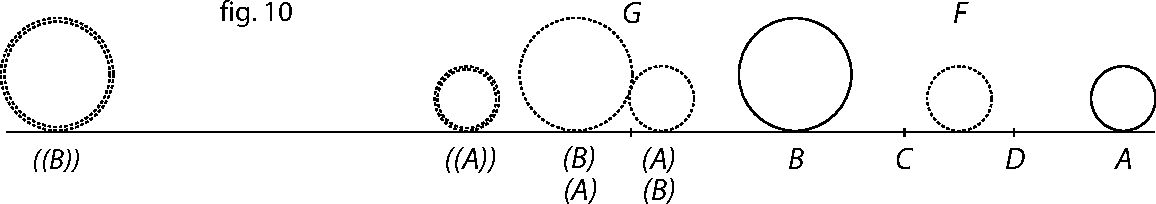
\includegraphics[width=1.0\textwidth]{gesamttex/edit_VIII,3/images/LH_35_09_23_011-012_d.pdf}}%
  \vspace{0.5em}
  \centerline{\lbrack\textit{Fig.~1}\rbrack}%
  \label{LH_35_09_23_011r_Fig.1}%
%  \vspace{0.75em}%
  \newpage%
%
\pstart%
Porro%
\edlabel{LH_35_09_23_011r_ghudr-2}%
\edlabel{LH_35_09_23_011r_ersteMarg_ytv-2}
%
\textit{(B)((B))} aequ.
%
\edtext{\textit{y},
et}{%
\lemma{\textit{y},}\Bfootnote{%
\textit{(1)}~aequ.
\textit{(2)}~et%
~\textit{L}}}
%
$by+a\epsilon\,\sqcap\,bi+ae,$
est autem $a\epsilon\,\sqcap\, 2ai-ae-\displaystyle\frac{a^2}{b}\overline{e-i}.$
\rule[-2mm]{0pt}{7mm}%
Ergo
\textit{by} aequ. $bi+ae-2ai+ae+\displaystyle\frac{a^2}{b}\,\overline{e-i},$
\rule[-2mm]{0pt}{0mm}%
seu
\textit{by} aequ. $bi+2ae-2ai+\displaystyle\frac{a^2}{b}\,\overline{e-i}.$
\rule[-2mm]{0pt}{0mm}%
Ergo fiet
\textit{y} aequ.
\rule[-2mm]{0pt}{7mm}%
%
% \edtext{%
$i,\!,+ \overline{\displaystyle\frac{2a}{b}+\displaystyle\frac{a^2}{b^2}},\overline{e-i}.$
% }{%
% \lemma{$i,\!,+ \overline{\displaystyle\frac{2a}{b}+\displaystyle\frac{a^2}{b^2}},\overline{e-i}$}\Cfootnote{%
% Richtig wäre:
% $y = i + \displaystyle\frac{a(2 - a)}{b(1 + b)}(e - i).$}}
%
Hinc si ad \textit{y} adderetur $e-2i$
fieret $y+e-2i$ aequ.
$\overline{e-i}, \,\overline{\framebox{2}\;\overline{1+\displaystyle\frac{a}{b}}},$%
\rule[-2mm]{0pt}{7mm}
seu fiet:
$y - i,\!,\, +\ e - i\ \text{aequ.}\
e - i, \overline{\framebox{2}\;1+\displaystyle\frac{a}{b}},$%
\rule[-3mm]{0pt}{9mm}
seu fiet:
$y-i$ aequ.
$\overline{\overline{\framebox{2}\;1+\displaystyle\frac{a}{b}},-1},\!,\overline{e-i},$
et $i-\epsilon$ aequ. $\overline{1+\displaystyle\frac{a}{b}},\!,\overline{e-i}.$%
\rule[-2mm]{0pt}{7mm}%
%
\edtext{}{%
\lemma{\textit{Am Rand:}}\Afootnote{% $\displaystyle\frac{y-i}{i-\epsilon}$
% \hspace{-0,5mm}%
% \lbrack...\rbrack\
% $\overline{+\displaystyle\frac{b}{b+a}+1}$
% \textit{erg.~L}
$\displaystyle\frac{y-i}{i-\epsilon}$ aequ. $\displaystyle\frac{1+\displaystyle\frac{a}{b}}{1}-\displaystyle\frac{1}{1+\displaystyle\frac{a}{b}}$ aequ. $\displaystyle\frac{b+a}{b}-\displaystyle\frac{b}{b+a}$ seu $\displaystyle\frac{y-i}{i-\epsilon}$ aequ. $\displaystyle\frac{b^2+2ab+a^2-b^2}{b^2+ab}$ aequ. $\displaystyle\frac{2ab+a^2}{b^2+ab}$ aequ. $\displaystyle\frac{a}{b},\displaystyle\frac{\overline{+2b+a}}{b+a}$ aequ. $\displaystyle\frac{a}{b},\overline{+\displaystyle\frac{b}{b+a}+1}.$%
\newline%
}}
%
Ergo addendo
$y-i$ et $i-\epsilon,$
fiet:
$y-\epsilon$ aequ.
\rule[-2mm]{0pt}{7mm}%
$\overline{\framebox{2}\;\overline{1+\displaystyle\frac{a}{b}},+\displaystyle\frac{a}{b}},\!,\overline{e-i}$%
\rule[-2mm]{0pt}{7mm}
%
\edtext{%
seu
$\overline{1+\displaystyle\frac{3a}{b}+\displaystyle\frac{a^2}{b^2}},\!,\overline{e-i},$%
}{\lemma{\textit{Am Rand, nachträglich hinzugefügt:}}\Afootnote{%
$\displaystyle%
\frac{\displaystyle%
\efrac{\displaystyle%
b^2+3ab+a^2}%
{\displaystyle%
\hfill b-a\phantom{i}}}%
{\displaystyle%
\efrac{\displaystyle%
\phantom{b^3}\phantom{3}-ab^2-3a^2b-a^3}%
{\displaystyle%
\frac{\displaystyle%
b^3+3ab^2\phantom{3}+a^2b\phantom{-a^3}}%
{\displaystyle%
\phantom{'}b^3+2ab^2-2a^2b-a^3}}}$
% \newline%
}}%
\rule[-2mm]{0pt}{7mm}
%
\edtext{quae quantitas
$y-\epsilon$
est distantia corporum%
\protect\index{Sachverzeichnis}{distantia corporum}
seu \textit{((A))((B))}.}{%
\lemma{quae}\Bfootnote{\hspace{-0,5mm}%
quantitas \lbrack...\rbrack\ seu \textit{((A))((B))}
\textit{erg.~L}}}
%
Et si ponas
$e-i$ esse unitatem,%
\protect\index{Sachverzeichnis}{unitas}
quod semper fieri potest
\rule[-2mm]{0pt}{7mm}%
sumendo pro mensura,%
\protect\index{Sachverzeichnis}{mensura}
fiet:
$y-\epsilon$ aequ.
\rule[-2mm]{0pt}{7mm}%
$1+\displaystyle\frac{3a}{b} +
\edlabel{LH_35_09_23_011r_kouk-1}%
\frac{a^2}{b^2},$%
%
\edtext{}{%
{\xxref{LH_35_09_23_011r_kouk-1}{LH_35_09_23_011r_kouk-2}}%
{\lemma{$\displaystyle\frac{a^2}{b^2}$}\Bfootnote{%
\textit{(1)}~. Hinc patet et casus
\textit{(2)}~, et secundum \lbrack...\rbrack\ patet et
\textit{(a)}~quando fit 1
\textit{(b)}~ponendo $\displaystyle\frac{a}{b}$ aequ. $\bigodot,$ quando fit
\lbrack...\rbrack\ aequ.~0,
\textit{(aa)}~fieri rep
\textit{(bb)}~corpora duo eadem celeritate progredi,%
~\textit{L}}}}
%
et secundum hunc considerandi modum%
\protect\index{Sachverzeichnis}{modus considerandi}
iisdem numeris exprimentur omnes differentiae,
$y-\epsilon,$
quando corpora \textit{a},
\textit{b} eadem manent.%
\rule[-2mm]{0pt}{7mm}
\pend%
% \newpage%
%
\pstart%
Hinc patet et
ponendo $\displaystyle\frac{a}{b}$
aequ. $\bigodot,$
quando fit:
% \rule[-3mm]{0pt}{9mm}%
$1+3\bigodot+\bigodot{}^2$
%
aequ.~0,
corpora duo eadem celeritate progredi,%
\protect\index{Sachverzeichnis}{celeritas progressus}%
\edlabel{LH_35_09_23_011r_kouk-2}
seu simul,
verum cum aequatio haec sit impossibilis,%
\protect\index{Sachverzeichnis}{aequatio impossibilis}
etiam casus iste erit impossibilis.%
\protect\index{Sachverzeichnis}{casus impossibilis}
$y-\epsilon$ est distantia corporum%
\protect\index{Sachverzeichnis}{distantia corporum}%
\rule[-2mm]{0pt}{8mm}
in casu progressus incurrentis,%
\protect\index{Sachverzeichnis}{casus progressus}%
\protect\index{Sachverzeichnis}{progressus corporis incurrentis}
nempe
$\overline{1+\displaystyle\frac{3a}{b}+\displaystyle\frac{a^2}{b^2}},\!,%
\edlabel{LH_35_09_23_011_rgtj-1}%
\overline{e-i}$%
\rule[-3mm]{0pt}{9mm}%
\edtext{}{%
{\xxref{LH_35_09_23_011_rgtj-1}{LH_35_09_23_011_rgtj-2}}%
{\lemma{$\overline{e-i}$}\Bfootnote{%
\textit{(1)}~aequ.
\textit{(2)}~seu $y-\epsilon$
\textit{(3)}~seu $y-\epsilon$ aequ.%
~\textit{L}}}}
%
% \pend%
% \vspace{0.75em}%
%
% \pstart%
% \noindent%
% \quad%
\,\lbrack\textit{Nachfolgend kleingedruckter Text in~L gestrichen:}\rbrack\
% \pend%
% \vspace{0.25em}%
%
{\footnotesize%
% \pstart%
% \noindent%
\edtext{%
seu
$y-\epsilon$
aequ.%
\edlabel{LH_35_09_23_011_rgtj-2}
$\displaystyle\frac{b^3+a^3}{b^2,a+b},e-i,$
seu
$\displaystyle\frac{y-\epsilon}{e-i}$
aequ.
%
\edtext{$\displaystyle\frac{a^3+b^3}{b^2,a+b}$
seu distantia posterioris est ad priorem,%
\protect\index{Sachverzeichnis}{distantia corporum}}{%
\lemma{$\displaystyle\frac{a^3+b^3}{b^2,a+b}$}\Bfootnote{%
\hspace{-0,5mm}seu
\textit{(1)}~differentia
\textit{(2)}~distantia
\textit{(a)}~corporum
\textit{(b)}~posterioris est ad priorem,%
~\textit{L}}}
%
ut summa cuborum corporum%
\protect\index{Sachverzeichnis}{summa corporum}
ad factum
ex quadrato majoris%
\protect\index{Sachverzeichnis}{corpus majus}
in amborum summam.%
\protect\index{Sachverzeichnis}{summa corporum}%
}{\lemma{{\normalsize{\textit{Am Rand, gestr.:}}}}\Afootnote{%
{\footnotesize%
$\displaystyle%
\frac{\displaystyle%
\efrac{\displaystyle%
b^2 \,[-\, ab]\textsuperscript{[a]} +a^2}{\displaystyle%
\hfill b + a\phantom{g}}}%
{\efrac{\displaystyle%
\hfill\phantom{+\;b^3}\protect\vphantom{a^{l}} +ab^2 -a^2b +a^3}%
{\displaystyle%
\frac{\displaystyle%
+\,b^3 -ab^2 +a^2b \phantom{+\,a^3}}%
{\displaystyle%
\phantom{+\ }b^3\protect\vphantom{b^3} % \hfill 
\phantom{+ab^2\; -a^2b\;} +a^3}}}$
\newline%
\newline%
\textsuperscript{[a]}~$+\,$\textit{ab} \textit{L~ändert Hrsg.}\vspace{-0.5em}
%
}}}%
}
%
%\edtext{}{%
%\lemma{\textit{Am Rand:}}\Afootnote{%
%$\displaystyle%
%\frac{\displaystyle\efrac{\displaystyle\frac{\displaystyle\efrac{b^2+3ab+a^2}{\hfill b-a}}{\phantom{b^3}-\phantom{3}ab^2-3a^2b-a^3}}{b^3+3ab^2+\phantom{2}a^2b\phantom{-a^3}}}{b^3+2ab^2-2a^2b-a^3}$\textsuperscript{[a]}
%\newline%
%\newline%
%{\footnotesize%
%\textsuperscript{[a]}
%\textit{(1)}~$\displaystyle\frac{\displaystyle\efrac{\displaystyle\frac{\hfill\displaystyle\efrac{b^2+ab+a^2}{\hfill b+a}}{\phantom{nb^3}+ab^2-a^2b\phantom{+}a^3}}{+b^3-ab^2+a^2b\phantom{na^3}}}{\phantom{+}b^3\phantom{+nab^2}\phantom{na^2b}+a^3}$
%\textit{(2)}~$\displaystyle\frac{\displaystyle\efrac{\displaystyle\frac{\hfill\displaystyle\efrac{b^2+3ab+a^2}{\hfill b-a}}{\phantom{b^3}-\phantom{3}ab^2-3a^2b-a^3}}{b^3+3ab^2+\phantom{2}a^2b\phantom{+na^3}}}{b^3+2ab^2-2a^2b-a^3}$%
%~\textit{L}}}}
%
% \quad%
\,{\normalsize%
\lbrack11~v\textsuperscript{o}\rbrack\ \,% % % %   Blatt 11v
}%
% \pend%
% \vspace{1.0em}
% \newpage%
%
% \normalsize%
% \pstart%
% \noindent%
\,$y-\epsilon$ aequ $\overline{1+\displaystyle\frac{3a}{b}+\displaystyle\frac{a^2}{b^2}},\overline{e-i}.$
\rule[-2mm]{0pt}{7mm}%
Ergo
$\displaystyle\frac{y-\epsilon}{e-i} \sqcap \displaystyle\frac{b^2+3ba+a^2}{b^2},$
seu
\rule[-2mm]{0pt}{7mm}%
$\displaystyle\frac{y-\epsilon}{e-i} \sqcap \framebox{2}\, \displaystyle\frac{b+a}{b},\!,
\edtext{[+\,\displaystyle\frac{a}{b}]}{%
\lemma{$-\,\displaystyle\frac{a}{b}$}\Bfootnote{%
\textit{L~ändert Hrsg.}}}.$
\rule[-2mm]{0pt}{7mm}%
\pend%
%
\pstart%
Via centri est%
\protect\index{Sachverzeichnis}{via centri gravitatis}%
\protect\index{Sachverzeichnis}{centrum gravitatis}
$\displaystyle\frac{a}{a+b}\overline{e-i}+i$
aequ.
\rule[-2mm]{0pt}{7mm}%
%
$\edtext{\displaystyle\frac{ae+ai}{a+b}}{%
\lemma{$\displaystyle\frac{ae+ai}{a+b}$}\Cfootnote{%
Die Herleitung ist falsch.
Richtig wäre: $\displaystyle\frac{ae + bi}{a + b}.$
Der Fehler wirkt sich auf die weiteren Herleitungen bis zum Ende des Absatzes aus.
Weitere Herleitungsfehler reihen sich an.}}%
%
\sqcap%
\displaystyle\frac{a}{a+b}\overline{e+i},$
quae si auferatur ab
$y - \epsilon$
seu a
\rule[-3mm]{0pt}{9mm}%
$\displaystyle\frac{\framebox{3}\;\overline{b+a},\!, +\, ba,\overline{a+b}}{b^2,a+b},$
seu scribatur
$y-\epsilon,\!,\, -$
via centri,%
\protect\index{Sachverzeichnis}{via centri gravitatis}
\!\raisebox{-1.5ex}{$\displaystyle\efrac{\textit{C(C)}}{\textit{C(B)}}$}$
\,\sqcap\;
\displaystyle\frac{\framebox{3}\;\overline{b+a},\!, +\, ba,a+b,\!,\, e-i}{b^2,\!,a+b},\!,$
$-ab^2,\!,\, e+i,$%
\rule[-2mm]{0pt}{7mm}
fiet
$y - \epsilon,\!,\, -$
via centri:
\rule[-2mm]{0pt}{7mm}%
$\displaystyle\frac{b^3e+a^3+2b^2ae+3ba^2e,\!,\, +b^3i+a^3i+2b^2ai+3ba^2i}{b^2,a+b},$%
\rule[-2mm]{0pt}{7mm}
seu si centrum gravitatis aequabiliter procederet,%
\protect\index{Sachverzeichnis}{centrum gravitatis}%
\rule[-2mm]{0pt}{7mm}
%
\edtext{foret distantia ejus}{%
\lemma{foret}\Bfootnote{%
\textit{(1)}~via
\textit{(2)}~distantia ejus%
~\textit{L}}}
%
a \textit{((B))},
sive
%
\edtext{\textit{((B))((C))} aequ.}{%
\lemma{\textit{((B))((C))}}\Bfootnote{\hspace{-0,5mm}%
\textbar~aequ. \textit{streicht Hrsg.}~%
\textbar~aequ.%
~\textit{L}}}
%
\rule[-2mm]{0pt}{7mm}%
$\displaystyle\frac{\framebox{3}\;\overline{b+a},\!,\,\overline{e-i}+ba^2,\overline{e-i},-\,2ab^2i}{b^2,a+b},$
sed falsa haec aequatio,%
\protect\index{Sachverzeichnis}{aequatio falsa}
\edtext{ostendi enim
centrum gravitatis%
\protect\index{Sachverzeichnis}{centrum gravitatis}
non progredi%
\protect\rule[-0mm]{0pt}{4mm}%
\protect\index{Sachverzeichnis}{progressus centri gravitatis}
eodem modo.}{\lemma{ostendi \lbrack...\rbrack\ modo}\Cfootnote{%
Vgl. N.~\ref{dcc_02-1}, %??S01\textsubscript{2}, 
S.~\refpassage{LH_35_09_23_006r_viacentrigrav_vlai-1}{LH_35_09_23_006r_viacentrigrav_mesj-2};
N.~\ref{dcc_02-2}, %??S01\textsubscript{3},
S.~\refpassage{LH_35_09_23_004v_motusperpetuus_nnxh-1}{LH_35_09_23_004v_motusperpetuus_nnxh-2};
N.~\ref{dcc_03}, %??S01\textsubscript{4},
S.~\refpassage{LH_35_09_23_007r_viacentrigrav_dvte-1}{LH_35_09_23_007r_viacentrigrav_dvte-2}.%
}}
\pend%
\newpage%
%
\pstart%
Pro casu repulsae%
\protect\index{Sachverzeichnis}{casus repulsae}%
\protect\index{Sachverzeichnis}{repulsa}%
\lbrack,\rbrack\
similis calculus prodit,%
\protect\index{Sachverzeichnis}{calculus}
nempe \textit{(A)((A))} erit
\rule[-1mm]{0pt}{0mm}%
$\displaystyle\frac{b-a}{b},\overline{e-i},\!,-\,i$
aequ.
$\epsilon$ \rule[-3mm]{0pt}{7mm}%
%
\edtext{seu $e-2i-\displaystyle\frac{a}{b}e+\displaystyle\frac{a}{b}i$ seu $e-2i,-\displaystyle\frac{a}{b}\overline{e-i},$}{%
\lemma{seu}\Bfootnote{%
\hspace{-0,5mm}$e-2i-\displaystyle\frac{a}{b}e+\displaystyle\frac{a}{b}i$ seu $e-2i,-\displaystyle\frac{a}{b}\overline{e-i}$
\textit{erg.~L}}}
%
et $by+a\epsilon \sqcap ae+bi$ fiet:
\rule[-3mm]{0pt}{9mm}%
$y \sqcap \displaystyle\frac{ae+bi-a\epsilon}{b}\sqcap \displaystyle\frac{\left\{\displaystyle\efrac{+\,ae}{-\,a\epsilon}\right.}{b}+i$
et
\rule[-3mm]{0pt}{9mm}%
$y \sqcap +\, i +\ovalbox{$\displaystyle\frac{ae}{b}-\displaystyle\frac{a}{b}\epsilon$}+\displaystyle\frac{2a}{b}i+\displaystyle\frac{a^2}{b^2}\overline{e-i},$
\rule[-3mm]{0pt}{9mm}%
et $\epsilon +y$
seu distantia corporum nova erit:%
\protect\index{Sachverzeichnis}{distantia corporum nova}
\rule[-0mm]{0pt}{6mm}%
$e -
\!\!\raisebox{-1.8ex}{$\displaystyle\efrac{\ovalbox{$2$}\,i}{\,\ovalbox{$+\,i$}}$}\!
- \displaystyle\frac{a}{b}e
\!\raisebox{-2.6ex}{$\displaystyle\efrac{\displaystyle+\, \frac{a}{b}i}{+\, \displaystyle\frac{2a}{b}i}$}\!\!
+\displaystyle\frac{a^2}{e^2}\overline{e-i}.$%
\rule[-3mm]{0pt}{3mm}%
\edlabel{LH_35_09_23_011-012_11v1}%
\edtext{}{%
{\xxref{LH_35_09_23_011-012_11v1}{LH_35_09_23_011-012_11v2}}%
{\lemma{$+\displaystyle\frac{a^2}{e^2}\overline{e-i}.$}\Bfootnote{%
\textit{(1)}~(fig.~3)
\textit{(2)}~Vis \textit{ae}, \textit{bi}, ubi concurrent
\textit{(3)}~$\displaystyle\frac{ae}{a+b}$
\textit{(a)}~vis qua procederetur
\textit{(b)}~celeritas qua \lbrack...\rbrack\ in quiescens%
~\textit{L}}}}%
\edlabel{LH_35_09_23_011v_jbcagk}%
\pend%
\vspace{1.5em}%
%
\pstart%
\noindent%
\rule[-0mm]{0pt}{0mm}%
\edtext{$\displaystyle\frac{ae}{a+b}$
celeritas qua procederet%
\protect\index{Sachverzeichnis}{celeritas progressus}
%
corpus motum incurrens%
\protect\index{Sachverzeichnis}{corpus incurrens}
in quiescens%
\protect\index{Sachverzeichnis}{celeritas corporis incurrentis}%
\protect\index{Sachverzeichnis}{corpus quiescens}%
\edlabel{LH_35_09_23_011-012_11v2}
si nulla esset percussio.%
\protect\index{Sachverzeichnis}{percussio nulla}%
}{%
\lemma{$\displaystyle\frac{ae}{a+b}$ \lbrack...\rbrack\ percussio}\Cfootnote{%
Die bisherige Untersuchung (über den Fall eines kleineren Körpers, der auf einen größeren, sich in dieselbe Richtung fortbewegenden stößt) bricht hier ab
und wird,
wie Leibniz selbst in der Randbemerkung zu S.~\refpassage{LH_35_09_23_012r_marg_cnjz-1}{LH_35_09_23_012r_marg_cnjz-2} festhält,
durch eine neue Untersuchung ersetzt,
bei der die Wirkung der Elastizität beim Stoß im Mittelpunkt steht.
Ausgangspunkt ist jetzt wieder der Fall eines Körpers,
der in einen ruhenden stößt.
Diese neue Untersuchung knüpft an ältere Texte wie etwa N.~\ref{RK57266-1} an.% ??M01 = Elaterium causa imperfectionis 
}}
%
Ergo vis percussionis%
\protect\index{Sachverzeichnis}{vis percussionis}
%
\edtext{est
$ae \smallfrown 1-\displaystyle\frac{a}{a+b}
\,\sqcap\,
ae \smallfrown \displaystyle\frac{b}{a+b},$
quae detracta de \textit{ae},
relinquit
$ae,\; \smallfrown \displaystyle\frac{a}{a+b}$
quae tota transibit in corpus \textit{B},
praetereaque dimidia pars ejus
divisa per \textit{a},
scilicet $\displaystyle\frac{[a]}{2,a+b}e,$
detrahetur a celeritate ipsius \textit{A} residua,%
\protect\index{Sachverzeichnis}{celeritas residua}
seu a $\displaystyle\frac{a}{a+b}\protect\framebox{2},e.$%
}{%
\lemma{est}\Bfootnote{%
\textit{(1)}~$ae -\displaystyle\frac{ae}{a+b}$
\textit{(2)}~$ae \smallfrown 1-\displaystyle\frac{a}{a+b} \sqcap ae \smallfrown \displaystyle\frac{b}{a+b},$
\textit{(a)}~cujus dimidium $\displaystyle\frac{ab}{2,\overline{a+b}} \smallfrown e$ (\protect\vphantom)ni fallor medium harmonicum%
\protect\index{Sachverzeichnis}{medium harmonicum} inter~\textit{a} et~\textit{b}\protect\vphantom() quod divisum per \textit{a}, dabit $\displaystyle\frac{b}{2,a+b}e,$ quae quantitas
\textit{(b)}~et residua vis%
\protect\index{Sachverzeichnis}{vis residua}
\textit{(c)}~quae detracta % de \textit{ae}, relinquit $ae, \smallfrown \displaystyle\frac{a}{a+b}$ quae tota transibit in corpus \textit{B} praetereaque dimidia 
\lbrack...\rbrack\ pars ejus
\textit{(aa)}~detrahetur \textit{ae}
\textit{(bb)}~divisa per \textit{a}, scilicet
\textbar~$\displaystyle\frac{b}{2,a+b}e$
\textit{ändert Hrsg.}~%
\textbar\ detrahetur a % celeritate ipsius \textit{A} residua, seu 
\lbrack...\rbrack\ a $\displaystyle\frac{a}{a+b}\protect\framebox{2},e.$%
~\textit{L}}}
%
\pend%
%
\pstart%
Si nulla esset resistentia,%
\protect\index{Sachverzeichnis}{resistentia nulla}
foret celeritas post incursum%
\protect\index{Sachverzeichnis}{celeritas post incursum}
\rule[-2mm]{0pt}{7mm}%
$\displaystyle\frac{ae}{a+b}$
quae ducta in \textit{b},
dabit vim%
\protect\index{Sachverzeichnis}{vis corporis incurrentis}%
\protect\index{Sachverzeichnis}{vis communicata}%
\protect\index{Sachverzeichnis}{corpus incurrens}%
\protect\index{Sachverzeichnis}{corpus quiescens}
quam corpus incurrens quiescenti communicaret,
scilicet
\rule[-2mm]{0pt}{7mm}%
\edtext{$\displaystyle\frac{ab}{a+b}e$
(\protect\vphantom)%
$\displaystyle\frac{3}{2}$ dentur ipsi \textit{b},
movebitur%
\protect\vphantom()%
}{%
\lemma{$\displaystyle\frac{ab}{a+b}e$}\Bfootnote{%
\textit{(1)}~cujus
\textit{(2)}~(\protect\vphantom)$\displaystyle\frac{3}{2}$ dentur ipsi \textit{b}, movebitur\protect\vphantom()%
~\textit{L}}}
%
et restabit vis pro progressu%
\protect\index{Sachverzeichnis}{vis pro progressu}
\rule[-0mm]{0pt}{6mm}$%
ae-\displaystyle\frac{abe}{a+b}$
aequ.
\rule[-0mm]{0pt}{6mm}%
\edtext{$\displaystyle\frac{a^2e\;\protect\ovalbox{$-\,abe+abe$}}{a+b},$
sive
$\displaystyle\frac{a}{a+b}ae$
quae rursus divisa per $a+b$
dabit celeritatem communem%
\protect\index{Sachverzeichnis}{celeritas communis}
$\displaystyle\frac{a^2}{a^2+2ab+b^2}e,$%
}{%
\lemma{$\displaystyle\frac{a^2e\;\protect\ovalbox{$-abe+abe$}}{a+b},$}\Bfootnote{%
\textit{(1)}~seu $\displaystyle\frac{a}{a+b} \smallfrown e\displaystyle\frac{2a^2e+abe}{2,a+b}$ sive $ae+\displaystyle\frac{a}{2,a+b}e+\displaystyle\frac{ae}{2}$
\textit{(2)}~sive $\displaystyle\frac{a}{a+b}ae$
\textit{(a)}~celeritas communis, cui addatur $\displaystyle\frac{b}{a+b}ae$ celeritas
\textit{(b)}~quae rursus \lbrack...\rbrack\ communem $\displaystyle\frac{a^2}{a^2+2ab+b^2}e,$ %
~\textit{L}}}
%
cui addatur
$\displaystyle\frac{3}{2}
\displaystyle\frac{ab}{a+b}e$
divisa per \textit{b},
fiet
$\framebox{2}\displaystyle\frac{a}{a+b},e,\!,
+\,\displaystyle\frac{3a}{2,a+b},e$
celeritas excipientis.%
\protect\index{Sachverzeichnis}{celeritas corporis excipientis}%
\rule[-4mm]{0pt}{0mm}
%
\lbrack12~r\textsuperscript{o}\rbrack\ % % % % Blatt 12r
%
\pend%
%
\pstart
\textit{a} et \textit{b} aequalia sunto,%
\protect\index{Sachverzeichnis}{corpora aequalia}
%
et \textit{a} incurrat in \textit{b} quiescens,%
\protect\index{Sachverzeichnis}{corpus incurrens}%
\protect\index{Sachverzeichnis}{corpus quiescens}
% \edtext{}{%
% \lemma{et}\Bfootnote{%
% \textit{(1)}~concurran
% \textit{(2)}~\textit{a} incurrat in \textit{b} quiescens%
% ~\textit{L}}}
%
videamus quomodo inde
%
\edtext{quies.%
\protect\index{Sachverzeichnis}{quies}
%
\edtext{%
\edlabel{LH_35_09_23_012r_marg_cnjz-1}%
Certum esse arbitror
majorem esse percussionem,%
\protect\index{Sachverzeichnis}{percussio major}
cum duo corpora concurrant%
\protect\index{Sachverzeichnis}{corpora concurrentia}
vi inter ipsa aequaliter partita,%
\protect\index{Sachverzeichnis}{vis aequaliter partita}
quam quando vis in uno tantum est,
alterum vero quiescit.%
\protect\index{Sachverzeichnis}{corpus quiescens}
Percussio%
\protect\index{Sachverzeichnis}{percussio}
videtur esse tanta
quanta est resistentia.%
\protect\index{Sachverzeichnis}{resistentia}%
\edlabel{LH_35_09_23_012r_marg_cnjz-2}%
}{%
\lemma{\textit{Am Rand:}}\Afootnote{%
Hae ratiocinationes%
\protect\index{Sachverzeichnis}{ratiocinatio de vi elastica}
de vi Elastica%
\protect\index{Sachverzeichnis}{vis elastica}
interrumpunt seriem praecedentium ratiocinationum%
\protect\index{Sachverzeichnis}{series ratiocinationum}
et\textsuperscript{[a]} probandae sunt magna ex parte.
\newline\vspace{-0.4em}%
\newline%
{\footnotesize%
\textsuperscript{[a]}~et
\textit{(1)}~pleraeque
\textit{(2)}~probandae sunt magna ex parte.%
~\textit{L}%
%\newline%
}}}%
%
}{%
\lemma{quies}\Bfootnote{%
\textit{(1)}~: resistentia est incurrentis
\textit{(2)}~. Resistentia incurrentis
\textit{(3)}~. Certum esse \lbrack...\rbrack\ est resistentia.%
~\textit{L}}}
%
\pend%
%
\pstart%
Si manente corpore excipiente%
\protect\index{Sachverzeichnis}{corpus excipiens}
%
\edtext{et manente celeritate incursus%
\protect\index{Sachverzeichnis}{celeritas incursus}%
\protect\index{Sachverzeichnis}{incursus}%
}{%
\lemma{et}\Bfootnote{%
\hspace{-0,5mm}manente celeritate incursus
\textit{erg.~L}}}
%
augeatur incurrens,%
\protect\index{Sachverzeichnis}{corpus incurrens}
quaeritur an augeatur percussio?%
\protect\index{Sachverzeichnis}{percussio aucta}
Ita certe.
\pend%
\vspace{0.5em}%
%
\pstart%
\noindent%
\lbrack\textit{Nachfolgend kleingedruckter Text in L gestrichen:}\rbrack\
\pend%
\vspace{0.5em}%
%
\footnotesize%
\pstart%
% \noindent%
Quaeritur an dividenda vis in duas partes,
unaque earum tribuenda percussioni,%
\protect\index{Sachverzeichnis}{vis percussioni tribuenda}
ut $\displaystyle\frac{ae}{2},$
qua corpora se conantur separare.%
\protect\index{Sachverzeichnis}{conatus separationis}
%
\edtext{Ergo cuilibet}{%
\lemma{Ergo}\Bfootnote{%
\textit{(1)}~$\displaystyle\frac{3ae}{\phantom{3ae}}$
\textit{(2)}~cuilibet%
~\textit{L}}}
%
eorum dabitur $\displaystyle\frac{ae}{4},$
sed quia incurrens%
\protect\index{Sachverzeichnis}{corpus incurrens}
id recipere non potest,
imo regressu hoc%
\protect\index{Sachverzeichnis}{regressus}
etiam de suo perdit,
ideo excipiens%
\protect\index{Sachverzeichnis}{corpus excipiens}
recipiet $\displaystyle\frac{3}{4}ae,$
et praeterea $\displaystyle\frac{ab}{a+b}e$
quod debet esse
\edtext{non majus}{%
\lemma{non}\Bfootnote{%
\hspace{-0,5mm}majus
\textit{erg.~L}}}%
\lbrack,\rbrack\
%
minus quam $\displaystyle\frac{1}{4}ae$
seu $\displaystyle\frac{b}{a+b} \,\kleiner\, \displaystyle\frac{1}{4}$ seu $4b \;\kleiner\, a+b.$
Haec ergo raciocinatio inepta.%
\protect\index{Sachverzeichnis}{ratiocinatio inepta}
\pend%
\vspace{0.5em}%
%
\normalsize%
\pstart%
% \noindent%
Vis percussionis%
\protect\index{Sachverzeichnis}{vis percussionis seu elastica}
seu elastica%
\protect\index{Sachverzeichnis}{vis elastica}
an necessario inter duo corpora
aequaliter dividitur?
%
Imo quid si tantum agat in debilius?
\pend%
%\vspace{0.5em}%
\newpage%
%
\pstart%
\noindent%
\lbrack\textit{Nachfolgend kleingedruckter Text in L gestrichen:}\rbrack\
\pend%
\vspace{0.5em}%
%
\footnotesize%
\pstart%
% \noindent%
\edtext{%
Videndum
an dici possit
vim percussionis%
\protect\index{Sachverzeichnis}{vis percussionis}
esse eandem
pro quantitate appropinquationis%
\protect\index{Sachverzeichnis}{quantitas appropinquationis}
manente eadem.
Quod sane satis probabile videtur.
Et certe videtur vis corporum%
\protect\index{Sachverzeichnis}{vis corporum concurrentium}
in se invicem hinc esse aestimanda.%
\protect\index{Sachverzeichnis}{vis aestimanda}
Cum revera motus nil sit
nisi respectivum aliquid.%
\protect\index{Sachverzeichnis}{motus respectivus}%
\protect\index{Sachverzeichnis}{respectivum aliquid}%
}{%
\lemma{\textit{Am Rand:}}\Afootnote{%
Ratiocinemur paulo accuratius de vi percussionis.%
\protect\index{Sachverzeichnis}{vis percussionis}%
%\newline
}}
\pend%
\vspace{0.5em}%
%
\normalsize%
\pstart%
\noindent%
Sit ergo corpus \textit{a} incurrens%
\protect\index{Sachverzeichnis}{corpus incurrens}
%
\edtext{in aliud}{%
\lemma{in}\Bfootnote{%
\textit{(1)}~minus quiescens
\textit{(2)}~aliud%
~\textit{L}}}
%
\textit{b}.
Celeritas%
\protect\index{Sachverzeichnis}{celeritas concursus}
\textit{a} sit \textit{e}
%
\edtext{et \textit{b} sit \textit{i}}{%
\lemma{et \textit{b}}\Bfootnote{%
\hspace{-0,5mm}sit \textit{i}
\textit{erg.~L}}}
%
et percussio%
\protect\index{Sachverzeichnis}{percussio}
sit $p^2.$
Erit residua vis%
\protect\index{Sachverzeichnis}{vis residua}
$ae+bi-p^2$
quae divisa per $a + b$ dabit
$\displaystyle\frac{ae+bi-p^2}{a+b}$
celeritatem%
\protect\index{Sachverzeichnis}{celeritas progressus}
qua ambo corpora progredi conantur.%
\protect\index{Sachverzeichnis}{conatus progressionis}
Porro vis percussionis $p^2$%
\protect\index{Sachverzeichnis}{vis percussionis aequaliter distributa}
%
\edtext{in}{%
\lemma{in}\Bfootnote{
\textit{erg.~L}}}
%
corpora aequaliter distribuitur,
%
%\edtext{\lbrack distribuatur\rbrack,}{%
%\lemma{distribuitur}\Bfootnote{%
%\textit{L~ändert Hrsg.}}}
%
erit ergo pro corpore \textit{A}
ea vis%
\protect\index{Sachverzeichnis}{vis percussionis aequaliter distributa}
$\displaystyle\frac{p^2}{2},$
et celeritas%
\protect\index{Sachverzeichnis}{celeritas repulsae}
qua corpus \textit{A} repelletur
erit
\rule[-3mm]{0pt}{7mm}%
\edtext{$\displaystyle\frac{p^2}{2a}.$
Ergo si
$\displaystyle\frac{ae+bi-p^2}{a+b}$
aequ. $\displaystyle\frac{p^2}{2a}$}{%
\lemma{$\displaystyle\frac{p^2}{2a}.$}\Bfootnote{%
\textit{(1)}~Ergo si $\displaystyle\frac{ae-p^2}{a+b}$ aequ. $\displaystyle\frac{p^2}{2a},$ seu si $2a^2e-2ap^2$ aequ. $ap^2+bp^2,$
\textbar~seu si $2a^2e$ aequ. $3ap^2+bp^2$ \textit{erg.}~\textbar\
\textit{(2)}~Ergo si $\displaystyle\frac{ae+bi-p^2}{a+b}$ aequ. $\displaystyle\frac{p^2}{2a}$%
~\textit{L}}}
%
corpus \textit{A} quiescet,%
\protect\index{Sachverzeichnis}{corpus quiescens}
seu si vis residua post percussionem%
\protect\index{Sachverzeichnis}{vis residua post percussionem}%
\protect\index{Sachverzeichnis}{percussio}
sit ad vim percussionis%
\protect\index{Sachverzeichnis}{vis percussionis}
ut summa corporum%
\protect\index{Sachverzeichnis}{summa corporum}
ad duplum alicujus ut \textit{A},
\rule[-3mm]{0pt}{7mm}%
corpus \textit{A} quiescet,%
\protect\index{Sachverzeichnis}{corpus quiescens}
ut patet\lbrack,\rbrack\
\rule[-3mm]{0pt}{7mm}%
\edtext{seu
%\edtext{%
$p^2 \sqcap \displaystyle\frac{\overline{ae+bi},2a}{3a+b}.$%
%}{%
%\lemma{$p^2 \sqcap \displaystyle\frac{\overline{ae+bi},2a}{3a+b}$}\Cfootnote{%
%Die Herleitung ist falsch.
%Der richtige Wert für $p^2$ wäre: $\displaystyle\frac{2a\,(ae + bi - p^2)}{a+b}.$ Der Fehler wirkt sich auf die folgenden Herleitungen bis S.~\refpassage{}{}.???}}%
}{%
\lemma{seu}\Bfootnote{%
\hspace{-0,5mm}$p^2 \sqcap \displaystyle\frac{\overline{ae+bi},2a}{3a+b}$
\textit{erg.~L}}}
% \pend%
% %
% \pstart%
%
\edtext{Hinc conferendo}{%
\lemma{Hinc}\Bfootnote{%
\textit{(1)}~sumendo
\textit{(2)}~conferendo%
~\textit{L}}}
%
quando in superioribus%
\rule[-3,5mm]{0pt}{7mm}
%
\edtext{corpus aliquod%
\protect\index{Sachverzeichnis}{corpus quiescens}
quiescere diximus,}{%
\lemma{corpus}\Bfootnote{%
\textit{(1)}~incurrens
\textit{(2)}~aliquod
\textit{(a)}~quiescit inveniemus
\textit{(b)}~quiescere diximus,%
~\textit{L}}}
%
inde ducemus
qualis in illis casibus
fuerit vis percussionis.%
\protect\index{Sachverzeichnis}{vis percussionis}%
\rule[-3mm]{0pt}{7mm}%
\pend%
%
\pstart%
Nimirum
\edtext{quando corpora sunt aequalia,%
\protect\index{Sachverzeichnis}{corpora aequalia}%
\protect\index{Sachverzeichnis}{casus corporum aequalium}
et
%
\edtext{excipiens%
\protect\index{Sachverzeichnis}{corpus excipiens}%
\protect\index{Sachverzeichnis}{corpus quiescens}
quie\textls{vit},}{%
\lemma{excipiens}\Bfootnote{%
\textit{(1)}~quie\textls{scit}
\textit{(2)}~quie\textls{vit}%
~\textit{L}}}
%
etiam incurrens%
\protect\index{Sachverzeichnis}{corpus incurrens}%
\protect\index{Sachverzeichnis}{corpus quiescens}
quie\textls{scet}.%
}{\lemma{quando corpora \lbrack...\rbrack\ incurrens quie\textls{scet}}\Cfootnote{%
Vgl. N.~\ref{dcc_01}, %??S01\textsubscript{1},
S.~\refpassage{LH_35_09_23_001r_incurr-in-aequ-quiesc-1}{LH_35_09_23_001r_incurr-in-aequ-quiesc-2}
sowie
N.~\ref{dcc_04}, %??S01\textsubscript{5},
S.~\refpassage{LH_35_09_23_010r_elegansprop_cfjg-1}{LH_35_09_23_010r_elegansprop_cfjg-2}.%
}}
%
Est autem $p^2$ hoc casu
\rule[-3mm]{0pt}{7mm}%
$\displaystyle\frac{2a^2e}{3a+b},$
seu
$\displaystyle\frac{2a^2e}{4a}$
aequ.
\rule[-3mm]{0pt}{7mm}%
$\displaystyle\frac{ae}{2},$
id est vis percussionis%
\protect\index{Sachverzeichnis}{vis percussionis dimidia}
fuit dimidia totius
quae hoc loco erat \textit{ae}.%
\rule[-3mm]{0pt}{7mm}
%
\edlabel{LH_35_09_23_012r_aliuscasus_rubz-1}%
Quaeramus alium casum,%
\protect\index{Sachverzeichnis}{casus concursus}%
%
\edtext{}{%
{\xxref{LH_35_09_23_012r_aliuscasus_rubz-1}{LH_35_09_23_012r_aliuscasus_rubz-2}}%
{\lemma{Quaeramus \lbrack...\rbrack\ summam}\Cfootnote{%
Vgl. N.~\ref{dcc_04}, %??S01\textsubscript{5},
S.~\refpassage{LH_35_09_23_010r_elegansprop_cfjg-1}{LH_35_09_23_010r_elegansprop_cfjg-2}.
Die Wiedergabe ist allerdings fehlerhaft:
Leibniz rechnet hier (wohl versehentlich) mit $\displaystyle\frac{a}{b}$ statt $\displaystyle\frac{b-a}{b}.$}}}
%
supra ostendimus si corpus minus assequatur majus,%
\protect\index{Sachverzeichnis}{corpus minus in majus}
et sit celeritas minor%
\protect\index{Sachverzeichnis}{celeritas minor}
ad differentiam celeritatum,%
\protect\index{Sachverzeichnis}{differentia celeritatum}
ut cor-
\pend
\newpage
\pstart
\noindent pus minus ad corpus majus,%
\protect\index{Sachverzeichnis}{corpus minus}%
\protect\index{Sachverzeichnis}{corpus majus}
tunc corpus incurrens quiescet.%
\protect\index{Sachverzeichnis}{corpus incurrens}%
\protect\index{Sachverzeichnis}{corpus quiescens}
%
\rule[-3mm]{0pt}{7mm}%
Nimirum eo casu
$\displaystyle\frac{i}{e-i}$ aequ. $\displaystyle\frac{a}{b},$
seu
%
\edtext{%
\textit{bi} aequ. $ae - ai,$
seu
$\overline{a+b}\,i$
aequ. \textit{ae},}{%
\lemma{\textit{Am Rand:}}\Afootnote{%
$a+b$ aequ. $\displaystyle\frac{ae}{i},$
\textit{bi} aequ. $ae - ai$\vspace{-4mm}}}
%
seu
$\displaystyle\frac{i}{e}$
aequ.
% \rule[-3mm]{0pt}{7mm}%
$\displaystyle\frac{a}{a+b},$
seu celeritas minor ad majorem,%
\protect\index{Sachverzeichnis}{celeritas minor}%
\protect\index{Sachverzeichnis}{celeritas major}
ut corpus minus%
\protect\index{Sachverzeichnis}{corpus minus}
ad corporum summam.%
\protect\index{Sachverzeichnis}{summa corporum}%
\edlabel{LH_35_09_23_012r_aliuscasus_rubz-2}
\rule[-0mm]{0pt}{5mm}%
Ergo $i \sqcap \displaystyle\frac{ae}{a+b},$
%
\edtext{quem valorem%
\protect\index{Sachverzeichnis}{valor}
substituendo}{%
\lemma{quem valorem substituendo}\Cfootnote{%
Bei folgender Herleitung substituiert Leibniz unterschiedliche Werte, die er soeben aus dem Verhältnis $i : (e-i) = a : b$ gewonnen hat.}}
%
in
%
\edtext{aequ.}{\lemma{aequ.}\Cfootnote{%
\textit{aequationem}}}
%
$p^2$ aequ.
% \rule[0mm]{0pt}{0mm}%
%
\edtext{$\displaystyle\frac{\overline{ae+bi},2a}{3a+b}$
fiet ergo
$p^2$ aequ.
% \protect\rule[-3mm]{0pt}{9mm}%
$\displaystyle\frac{\overline{2ae-ai}}{2a+\displaystyle\frac{ae}{i}}\smallfrown 2a$
seu $p^2$ aequ.
% \protect\rule[-3mm]{0pt}{9mm}%
$\displaystyle\frac{4aei-2ai^2}{2i+e}.$%
}{%
\lemma{$\displaystyle\frac{\overline{ae+bi},2a}{3a+b}$}\Bfootnote{%
\textit{(1)}~fiet $\displaystyle\frac{2a^2e+\displaystyle\frac{2aeb}{a+b}}{3a+b},$ vel quia $a+b \sqcap \displaystyle\frac{ae}{i},$ substituendo in $p^2,$
\textit{(2)}~fiet
\textit{(a)}~: $\displaystyle\frac{\overline{ae+\overline{e-i}},a\displaystyle\frac{2a}{a+b}}{3a+a\smallfrown\displaystyle\frac{e-i}{i}}$ aequ. $p^2$ aequ. $\displaystyle\frac{\overline{2ei-i^2}2a}{\protect\ovalbox{3}\,i+e\,\protect\ovalbox{\!$-1$}}$ aequ. $\displaystyle\frac{2e-i}{2i+e}\smallfrown 2ai$
\textit{(b)}~ergo $p^2$ aequ.
\lbrack...\rbrack\ aequ. $\displaystyle\frac{4aei-2ai^2}{2i+e}.$%
~\textit{L}}}
%
\pend%
%
\pstart%
%
In casu quietis%
\protect\index{Sachverzeichnis}{casus quietis}
%
\edtext{$\displaystyle\frac{v^2-p^2}{a+b}$}{%
\lemma{$\displaystyle\frac{v^2-p^2}{a+b}$}\Cfootnote{%
Wie bereits in N.~\ref{RK57266-1},
%??M01 = Elaterium causa imperfectionis 
S.~\refpassage{LH_37_05_161v_setzungen-1}{LH_37_05_161v_setzungen-2}
stehen hier $v^2$ für die Summe der Bewegungsgröße ($ae + bi$)
und $p^2$ für die Stoßkraft (\textit{percussio}).
Siehe \textsc{Fichant} 1994, S.~112.\cite{01056}}}
%
aequ.
%
\edtext{$\displaystyle\frac{p^2}{2a}$
seu}{%
\lemma{$\displaystyle\frac{p^2}{2a}$}\Bfootnote{%
\textit{(1)}~\textbar~aequ. \textit{streicht Hrsg.}~\textbar\
\textit{(2)}~seu%
~\textit{L}}}
%
$\displaystyle\frac{v^2-p^2}{p^2} \sqcap \displaystyle\frac{a+b}{2a}$ seu $\displaystyle\frac{v^2}{p^2}-1$ aequ. $\displaystyle\frac{1}{2}+\displaystyle\frac{b}{2a},$ seu $\displaystyle\frac{v^2}{p^2} \sqcap \displaystyle\frac{3}{2}+\displaystyle\frac{b}{2a}.$
\pend%
%
\pstart%
In casu quietis
$\displaystyle\frac{2a}{a+b}
\sqcap \displaystyle\frac{p^2}{v^2-p^2}$
atqui in casu quietis%
\protect\index{Sachverzeichnis}{casus quietis}
cum corpus minus incurrit in majus antecedens,%
\protect\index{Sachverzeichnis}{corpus minus in majus}%
\protect\index{Sachverzeichnis}{corpus majus antecedens}
fit:
$\displaystyle\frac{2a}{a+b} \sqcap \displaystyle\frac{2i}{e}.$
\quad%
Ergo fit:
$\displaystyle\frac{p^2}{v^2-p^2}$
aequ.
$\displaystyle\frac{2i}{e}$
seu
$\displaystyle\frac{e}{2i}$
aequ.
$\displaystyle\frac{v^2}{p^2}-1$
aequ.
$\displaystyle\frac{b}{2a}+\displaystyle\frac{1}{2}.$
Seu
$\displaystyle\frac{v^2}{p^2}-\displaystyle\frac{b}{2a}
\,\sqcap\, \displaystyle\frac{3}{2}.$
\quad%
$\displaystyle\frac{2a}{a+b} \,\sqcap\, \displaystyle\frac{p^2}{v^2-p^2} \,\sqcap\, \displaystyle\frac{2i}{e}.$
\quad%
Ergo
$p^2 \,\sqcap\,
%
\displaystyle\frac{2v^2}{\displaystyle\frac{b}{a}+3}$
%
seu
$\sqcap\,
%
\displaystyle\frac{2a}{3a+b}v^2.$
%
$\displaystyle\frac{v^2}{p^2}-1 \,\sqcap\, \displaystyle\frac{e}{2i}.$
\quad%
Ergo
%
$p^2
\sqcap
\displaystyle\frac{v^2}{\displaystyle\frac{e}{2i}+1}
\sqcap
\edlabel{LH_35_09_23_012rv_fguh-1}%
\displaystyle\frac{2i}{e+2i}v^2.$%
%
\edtext{}{%
{\xxref{LH_35_09_23_012rv_fguh-1}{LH_35_09_23_012rv_fguh-2}}%
{\lemma{$\displaystyle\frac{2i}{e+2i}v^2.$}\Bfootnote{%
\hspace{-0,5mm}%
\textbar~Sed id hoc loco nec probare, nec refutare licet. \textit{gestr.}~%
\textbar\ \lbrack12~v\textsuperscript{o}\rbrack\ Ut% in universum
~\textit{L}}}}
%
\lbrack12~v\textsuperscript{o}\rbrack\ % % % %    Blatt 12v
%
\pend%
%\vspace{0.25em}%
\newpage
%
\pstart%
Ut in universum%
\edlabel{LH_35_09_23_012rv_fguh-2}
vim percussionis%
\protect\index{Sachverzeichnis}{vis percussionis}
investigem,
ita erit agendum.
Corpus aliquod amittit aliquid suae
%
\edtext{vis,%
\protect\index{Sachverzeichnis}{vis amissa}
idque}{%
\lemma{vis,}\Bfootnote{%
\textit{(1)}~vel
\textit{(2)}~idque%
~\textit{L}}}
%
tum ex eo,
quod corpus fortius%
\protect\index{Sachverzeichnis}{corpus fortius}%
\protect\index{Sachverzeichnis}{corpus abripiens}
abripit debilius,%
\protect\index{Sachverzeichnis}{corpus debilius}
sed minore celeritate,%
\protect\index{Sachverzeichnis}{celeritas minoris}
tum etiam ex repulsa ob percussionem,%
\protect\index{Sachverzeichnis}{repulsam ob percussionem}
itaque quicquid non perdidit ex abreptione,%
\protect\index{Sachverzeichnis}{abreptio}
id perdidit ex
%
\edtext{repulsa.%
\protect\index{Sachverzeichnis}{repulsa}
Nimirum}{%
\lemma{repulsa.}\Bfootnote{%
\textit{(1)}~Seu
\textit{(2)}~Nimirum%
~\textit{L}}}
%
abreptionis celeritas%
\protect\index{Sachverzeichnis}{celeritas abreptionis}
\rule[-0mm]{0pt}{5mm}%
\edtext{esset $\displaystyle\frac{ae}{a+b},$
quando corpus \textit{a}
incurrit in quiescens \textit{b}%
\protect\index{Sachverzeichnis}{corpus quiescens}
celeritate \textit{e},%
\protect\index{Sachverzeichnis}{celeritas incursus}
quae si substrahatur a celeritate \textit{e},}{%
\lemma{esset}\Bfootnote{%
\textit{(1)}~$\displaystyle\frac{ae+bi}{a+b},$ quando corpora non sibi occurrunt
\textit{(2)}~$\displaystyle\frac{ae}{a+b},$ quando
\textit{(a)}~corpus unum
\textit{(b)}~corpus \textit{a} incurrit in quiescens \textit{b}
\textit{(aa)}~, celeritas abrepti
\textit{(bb)}~celeritate \textit{e},
\textit{(aaa)}~et vis
\textit{(bbb)}~quae si substrahatur
\textit{(aaaa)}~ab \textit{a}
\textit{(bbbb)}~a celeritate \textit{e},%
~\textit{L}}}
%
restabit
$e-\displaystyle\frac{ae}{a+b},$
% \rule[-2mm]{0pt}{0mm}
id est
\rule[-3mm]{0pt}{0mm}%
%
$\displaystyle\frac{be}{a+b}
\edtext{\sqcap\ r.$
Quod si autem minus aliquid superest,
id periit per repercussionem.%
\protect\index{Sachverzeichnis}{repercussio}
Jam demonstravimus
\edtext{supra,}{%
\lemma{supra}\Cfootnote{%
Vgl. N.~\ref{dcc_01}, %??S01\textsubscript{1},
S.~\refpassage{LH_35_09_23_002r_majausinminus_bfnd-1}{LH_35_09_23_002r_majausinminus_bfnd-2}.%
%N.~\ref{dcc_02-1}, %??S01\textsubscript{2},
%S.~\refpassage{}{}.???
}}
si corpus aliquod \textit{a}
incurrat in quiescens \textit{b}%
\protect\index{Sachverzeichnis}{corpus quiescens}%
}{%
\lemma{$\sqcap\ r$}\Bfootnote{%
\textit{(1)}~quae foret celeritas perdita per percussionem. Ergo si
\textit{(a)}~corpus
\textit{(b)}~$\epsilon a$ ducta
\textit{(c)}~in \textit{a}
\textit{(2)}~. Quod si \lbrack...\rbrack\ quiescens \textit{b}%
~\textit{L}}}
%
et quidem majus in minus,%
\protect\index{Sachverzeichnis}{corpus majus in minus}
tunc celeritatem residuam%
\protect\index{Sachverzeichnis}{celeritas residua}
$\epsilon$ esse ad priorem \textit{e},
ut $a-b$ ad \textit{a},
seu%
\rule[-2mm]{0pt}{8mm}
$\epsilon \sqcap \displaystyle\frac{a-b}{a}e.$
Investigemus
%
\edtext{jam $r - \epsilon,$}{%
\lemma{jam}\Bfootnote{%
\textit{(1)}~$\epsilon - r$
\textit{(2)}~$r - \epsilon$%
~\textit{L}}}
%
fiet \protect\rule[-3mm]{0pt}{8mm}%
$\displaystyle\frac{be}{a+b}-\displaystyle\frac{a-b}{a}e$
aequ.%
\rule[-3mm]{0pt}{8mm}%
%
\edtext{$\displaystyle\frac{ab-a^2+b^2}{[a\,\overline{a+b}]}e,$}{%
\lemma{$a+b$}\Bfootnote{%
\textit{L~ändert Hsrg.}}}
%
\edtext{seu
$\protect\ovalbox{\textit{e}}\,-\displaystyle\frac{ae}{a+b},\!,\protect\ovalbox{$\!-\,e$}\,+\displaystyle\frac{b}{a}e.$%
\protect\rule[-3mm]{0pt}{8mm}
}{%
\lemma{\textit{Am Rand:}}\Afootnote{%
Notabile:
$\displaystyle\frac{be}{a+b} + \protect\ovalbox{$\displaystyle\frac{be}{a}$} - e$ aequ. $\protect\ovalbox{$\displaystyle\frac{be}{a}$}-\displaystyle\frac{ae}{a+b}.$
\newline%
}}
%
Ubi si ratiocinatio
ista proba est,%
\protect\index{Sachverzeichnis}{ratiocinatio proba}
necesse est
primum posito esse \textit{a}
majorem quam \textit{b},
semper
%
esse \textit{r}
%\edtext{}{%
%\lemma{esse}\Bfootnote{%
%\textit{(1)}~\textit{r}
%\textit{(2)}~\textit{e}
%\textit{(3)}~\textit{r}%
%~\textit{L}}}
%
majus quam $\epsilon,$
seu
\rule[-3mm]{0pt}{7mm}%
$\displaystyle\frac{b}{a+b}$
majus quam
\rule[-3mm]{0pt}{7mm}%
$\displaystyle\frac{a-b}{a},$
seu \textit{ab} majus
%
quam $\underbrace{a+b,\smallfrown a-b}_{\displaystyle a^2-b^2}.$
Scribatur
$a\, \sqcap\, b + \alpha$
%\edtext{}{%
%\lemma{quam}\Bfootnote{%
%\textit{(1)}~$ab \smallfrown$
%\textit{(2)}~$\underbrace{a+b,\smallfrown a-b}_{\displaystyle a^2-b^2}.$
%\textit{(a)}~Seu \textit{a}
%\textit{(b)}~Scribatur $a\, \sqcap\, b + \alpha$%
%~\textit{L}}}
%
fiet:
$ab\, \sqcap\, b^2 + \alpha b,$
et
$a^2 - b^2\, \sqcap\; \protect\ovalbox{$b^2\!$}\, + \alpha^2 + 2\alpha b\; \protect\ovalbox{$-\, b^2$}\,.$
%
\edtext{%
Ergo
$ab,-,\,\overline{\overline{a+b},\overline{a-b}}$
aequ.
$b^2\,\protect\ovalbox{$+\,\alpha b$}\,-\alpha^2%
%
\edtext{-\protect\ovalbox{$2$}\,\alpha b.$
Seu debet esse $b^2$ major quam $\alpha^2 + \alpha b,$}{%
\lemma{$-\,\protect\ovalbox{$2$}\,\alpha b$}\Bfootnote{%
\textit{(1)}~seu aequ. $2b^2 - a^2.$ Ergo necesse est $b\sqrt2$ esse majorem quam \textit{a}
\textit{(2)}~. Seu debet % esse $b^2$ major 
\lbrack...\rbrack\ quam $\alpha^2 + \alpha b,$%
~\textit{L}}}%
}{%
\lemma{\textit{Am Rand:}}\Afootnote{%
Seu
$+\,b^2 + b^2 - b^2 - \alpha^2 - 2$ \lbrack\textit{bricht ab.}\rbrack%
% \newline%
}}%
%
\rule[-3mm]{0pt}{4mm}
seu \textit{bb} major
%\edtext{}{%
%\lemma{seu}\Bfootnote{%
%\textit{(1)}~$b^2$ majo
%\textit{(2)}~\textit{bb} major%
%~\textit{L}}}
%
quam
%
\edtext{\lbrack$\alpha\alpha$\rbrack.}{%
\lemma{$a\alpha$}\Bfootnote{%
\textit{L~ändert Hrsg.}}}
%
Quod non est in potestate%
\protect\index{Sachverzeichnis}{potestas}
quia ipsae $\alpha$ et \textit{b}
sunt a se invicem independentes
et pro
\pend
\newpage
\pstart
\noindent
%
arbitrio sumi possunt,%
\protect\index{Sachverzeichnis}{arbitrium}
ergo potest contingere
ut $\alpha^2 + \alpha b$
non sit minor sed major \edtext{quam $b^2.$
Quo}{%
\lemma{quam $b^2.$}\Bfootnote{%
\textit{(1)}~Imo
\textit{(2)}~Quo%
~\textit{L}}}
%
casu residuum abreptionis \textit{r}%
\protect\index{Sachverzeichnis}{residuum abreptionis}%
\protect\index{Sachverzeichnis}{abreptio}
%
\edtext{est minus}{%
\lemma{est}\Bfootnote{\hspace{-0,5mm}%
\textbar~multo \textit{gestr.}~%
\textbar\ minus%
~\textit{L}}}
%
quam residuum abreptionis%
\protect\index{Sachverzeichnis}{residuum abreptionis}
simul et repercussionis;%
\protect\index{Sachverzeichnis}{repercussio}
cum tamen videatur id
quod a sola abreptione%
\protect\index{Sachverzeichnis}{abreptio}
relinquitur
semper debere esse majus
quam quod
%
\edtext{relinquitur ex duobus}{%
\lemma{relinquitur}\Bfootnote{%
\textit{(1)}~a sola
\textit{(2)}~ex duobus%
~\textit{L}}}
%
illis capitibus.%
\protect\index{Sachverzeichnis}{caput}
%
\edtext{%
Quae objectio%
\protect\index{Sachverzeichnis}{objectio difficilis}
nostras praecedentes ratiocinationes%
\protect\index{Sachverzeichnis}{ratiocinatio labefacta}
valde labefactaret.}{%
\lemma{\textit{Am Rand:}}\Afootnote{%
NB NB.
Objectio difficilis contra praecedentia.%
\protect\index{Sachverzeichnis}{objectio difficilis}
% \newline%
% \newline%
% \quad
\lbrack\textit{Hierzu, gestr.:}\rbrack\
{\footnotesize%
Nunc puto subesse errorem in calculo%
\protect\index{Sachverzeichnis}{error in calculo}
quoad objectionem.%
\newline%
}}}
\pend%
% \newpage%
%
\pstart%
Videamus tamen:
$b^2 + \beta^2 \,\sqcap\, \alpha^2 + \alpha b.$
Ergo
$b^2-\alpha b + \displaystyle\frac{\alpha^2}{4} \sqcap \displaystyle\frac{5}{4}\alpha^2-\beta^2.$
% \rule[-2mm]{0pt}{0mm}%
Ergo
$b-\displaystyle\frac{\alpha}{2} \sqcap \sqrt{\displaystyle\frac{5}{4}\alpha^2-\beta^2}.$
% \rule[-2mm]{0pt}{6mm}%
Seu $b \sqcap \sqrt{\displaystyle\frac{5}{4}\alpha^2-\beta^2}+\displaystyle\frac{\alpha}{2}.$
% \rule[-2mm]{0pt}{6mm}%
Et quies orietur,%
\protect\index{Sachverzeichnis}{quies orta}
quando
% \rule[-2mm]{0pt}{6mm}%
$b \sqcap \displaystyle\frac{\alpha}{2}\sqrt5 +\displaystyle\frac{\alpha}{2}.$
%
\edlabel{LH_35_09_23_012v_sbchj-1}%
Cum tamen nunquam quies oriri debeat%
\protect\index{Sachverzeichnis}{quies orta}
in casu incursus majoris in minus.%
\protect\index{Sachverzeichnis}{casus incursus}%
\protect\index{Sachverzeichnis}{corpus majus in minus}
Unde sequitur nos nondum satis exacte ratiocinatos,
dum
%
\edlabel{LH_35_09_23_012v_khtd-1}%
\edtext{lineam
%
\edtext{supra}{%
\lemma{supra}\Bfootnote{%
\textit{erg.~L}}}
%
supposuimus rectam.%
\protect\index{Sachverzeichnis}{linea recta}%
}{%
\lemma{lineam \lbrack...\rbrack\ rectam}\Cfootnote{%
Vgl.
N.~\ref{dcc_01}, %??S01\textsubscript{1},
S.~\refpassage{LH_35_09_23_002r_probaturrecta_mxyz-1}{LH_35_09_23_002r_probaturrecta_mxyz-2};
N.~\ref{dcc_02-1}, %??S01\textsubscript{2},
S.~\refpassage{LH_35_09_23_003v_recta_lje-1}{LH_35_09_23_003v_recta_lje-2};
N.~\ref{dcc_03}, %??S01\textsubscript{4},
S.~\refpassage{LH_35_09_23_007r_estrecta_jmgt-1}{LH_35_09_23_007r_estrecta_jmgt-2}.%
}}%
\edlabel{LH_35_09_23_012v_khtd-2}
% \pend%
%
% \pstart%
Seu cum
%
$ab\, \sqcap\,
\edtext{a^2 - b^2,$
seu cum
$b^2+ab+\displaystyle\frac{a^2}{4}
\sqcap
\displaystyle\frac{5}{4}a^2.$%
}{%
\lemma{$a^2 - b^2,$}\Bfootnote{%
\textit{(1)}~seu cum $b^2 + 2ab + a^2\ \sqcap\ 2a^2$
\textit{(2)}~seu cum $b^2+ab+\displaystyle\frac{a^2}{4} \sqcap \displaystyle\frac{5}{4}a^2.$%
~\textit{L}}}%
\rule[-2mm]{0pt}{7mm}
%
Seu cum
\rule[-2mm]{0pt}{7mm}%
$b+a\ \sqcap \displaystyle\frac{a}{2}\sqrt5.$%
\edlabel{LH_35_09_23_012v_sbchj-2}
%
%%%%%%%%%% Große Randbemerkung, Anfang <<<<
%
\edtext{}{%
{\xxref{LH_35_09_23_012v_sbchj-1}{LH_35_09_23_012v_sbchj-2}}%
{\lemma{\textit{Am Rand:}}\Afootnote{%
Hic certa demonstratione%
\protect\index{Sachverzeichnis}{demonstratio certa}
eversa est linea\textsuperscript{[a]}
recta qua usi eramus.%
\protect\index{Sachverzeichnis}{linea recta}
Quando corpus majus incurrit in minus%
\protect\index{Sachverzeichnis}{corpus majus in minus}%
\protect\index{Sachverzeichnis}{corpus quiescens}
quiescens\textsuperscript{[b]}
celeritas post incursum%
\protect\index{Sachverzeichnis}{celeritas post incursum}
minor est celeritate
qua ferrentur ambo simul,
si servata\textsuperscript{[c]}
quantitate virium%
\protect\index{Sachverzeichnis}{quantitas virium servata}
sese abriperent.
Ergo \textit{r} seu $\displaystyle\frac{be}{a+b}$
major quam $\epsilon,$
seu major quam
$\displaystyle\frac{a-b}{a}e,$
seu ergo
$\displaystyle\frac{b}{a+b}$
major quam $\displaystyle\frac{a-b}{a}.$
Positis scil. prioribus ratiocinationibus
seu $ab \;\groesser\; a^2 - b^2,$
seu posito
$a\ \text{aequ.}\ \alpha + b,$
fiet
$\alpha b + b^2 \,\groesser\,\alpha^2 + 2\alpha b\; \protect\ovalbox{$+\,b^2 - b^2$}$
seu
$b^2 \,\groesser\, \alpha^2 + \alpha b,$
quae patet semper non eventura.
Hinc ergo\textsuperscript{[d]}
errores superiores deprehendimus.%
\protect\index{Sachverzeichnis}{error deprehensus}
\newline%
\newline%
{\footnotesize%
\textsuperscript{[a]}~linea \lbrack...\rbrack\ eramus:
Siehe Erläuterung zu S.~\refpassage{LH_35_09_23_012v_khtd-1}{LH_35_09_23_012v_khtd-2}.
%
\quad
\textsuperscript{[b]}~quiescens
\textit{erg.~L}
\quad
\textsuperscript{[c]}~servata
\textit{(1)}~motus
\textit{(2)}~quantitate virium%
~\textit{L}
\quad
\textsuperscript{[d]}~ergo
\textit{(1)}~errorem
\textit{(2)}~errores%
~\textit{L}}%
%\newline%
}}}
%
%%%%%%%%%% Große Randbemerkung, Ende >>>>
%
\pend%
\newpage
\pstart%
Ponamus corpus aliquod moveri,%
%
\edtext{}{\lemma{\textit{Am Rand, gestr.:}}\Afootnote{%
{\footnotesize
Verissime.
 \newline%
}}}
%
eique inter procedendum imponi
%
\edtext{aliud corpus,
sine ulla percussione,%
\protect\index{Sachverzeichnis}{concursus sine percussione}
quaeritur an tunc minus impediatur,}{%
\lemma{aliud}\Bfootnote{%
\hspace{-0,5mm}corpus,
\textit{(1)}~utique minus imp
\textit{(2)}~sine ulla \lbrack...\rbrack\ minus impediatur%
~\textit{L}}}
%
quam si
\protect\index{Sachverzeichnis}{percussio}%
percussio fuisset
%
\edtext{secuta.
Et re accurate considerata
ita videtur,
non posse saltem plus efficere percussione,%
\protect\index{Sachverzeichnis}{percussio}
quam efficisset sine percussione.%
\protect\index{Sachverzeichnis}{concursus sine percussione}%
}{%
\lemma{secuta.}\Bfootnote{%
\textit{(1)}~Videtur sane per percussionem plus efficere
\textit{(2)}~Et re % accurate considerata ita videtur non posse saltem 
\lbrack...\rbrack\ plus efficere
\textit{(a)}~, quam effecisset
\textit{(b)}~percussione, quam efficisset sine percussione.%
~\textit{L}}}
%
\edtext{Itaque cum}{%
\lemma{Itaque}\Bfootnote{%
\textit{(1)}~in quantum
\textit{(2)}~cum%
~\textit{L}}}
%
\edtext{sine percussione secum abripiat corpus,%
\protect\index{Sachverzeichnis}{abreptio sine percussione}
nunc percussione ante se agat,}{%
\lemma{\textit{Am Rand:}}\Afootnote{%
Verissima.}}
%
\edtext{itaque primum necesse est,
ut}{%
\lemma{itaque}\Bfootnote{%
\textit{(1)}~conveniens videtur, ut
\textit{(2)}~primum necesse est, ut%
~\textit{L}}}
%
si corpus
in quod impingit%
\protect\index{Sachverzeichnis}{corpus impingens}
majore celeritate ante se agit
%
\edtext{quam qua movisset}{%
\lemma{quam}\Bfootnote{%
\textit{(1)}~quae erat
\textit{(2)}~qua movisset%
~\textit{L}}}
%
sine percussione,%
\protect\index{Sachverzeichnis}{percussio}
ut ipsum feratur,
minore quam qua tunc fuisset latum%
\lbrack,\rbrack\
alioqui vires%
\protect\index{Sachverzeichnis}{vis aucta}
%
\edtext{augerentur.
Et contra}{%
\lemma{augerentur.}\Bfootnote{%
\textit{(1)}~Sed
\textit{(2)}~Et contra%
~\textit{L}}}
%
si minore,
ipsum majore celeritate feretur.
Verum impossibile est
%
\edtext{ut corpus abripiens}{%
\lemma{ut}\Bfootnote{%
\hspace{-0,5mm}corpus
\textit{(1)}~incurrens
\textit{(2)}~abripiens%
~\textit{L}}}
%
aliud corpus cum%
\protect\index{Sachverzeichnis}{corpus abripiens cum percussione}
%
\edtext{percussione\lbrack,\rbrack\
progrediatur}{%
\lemma{percussione}\Bfootnote{%
\textit{(1)}~feratur
\textit{(2)}~progrediatur%
~\textit{L}}}
%
majore celeritate
quam abripiens ipsum sine percussione.%
\protect\index{Sachverzeichnis}{corpus abripiens sine percussione}
%
\edtext{Nam praeterquam
quod nulla ratio est,
quae faciat ut plus efficiat,
sequeretur absurdum,%
\protect\index{Sachverzeichnis}{absurdum}%
}{%
\lemma{Nam}\Bfootnote{%
\textit{(1)}~ergo et id quod secum impellit,
\textit{(a)}~feret
\textit{(b)}~ferretur majore celeri
\textit{(2)}~praeterquam quod \lbrack...\rbrack\ sequeretur absurdum%
~\textit{L}}}
%
nempe virium augmentum%
\protect\index{Sachverzeichnis}{augmentum virium}
in universum,%
\protect\index{Sachverzeichnis}{universum}
nam si abripiens citius fertur
etiam abreptum celerius fertur,%
\protect\index{Sachverzeichnis}{corpus abreptum}
ergo
%
major vis quam
%\edtext{}{%
%\lemma{major}\Bfootnote{%
%\textit{(1)}~quam
%\textit{(2)}~vis quam%
%~\textit{L}}}
%
si abfuisset percussio,%
\protect\index{Sachverzeichnis}{percussio}
ergo major vis quam ante concursum%
\protect\index{Sachverzeichnis}{vis ante concursum}
(\protect\vphantom)%
nam abreptio sine percussione%
\protect\index{Sachverzeichnis}{abreptio sine percussione}
servat eandem%
\protect\vphantom(),
quod absurdum.%
\protect\index{Sachverzeichnis}{absurdum}
\edlabel{LH_35_09_23_012v_subfine-1}%
Ergo abripiens cum percussione%
\protect\index{Sachverzeichnis}{corpus abripiens cum percussione}
non potest majori procedere celeritate%
\protect\index{Sachverzeichnis}{celeritas progressus}
quam abripiens sine percussione.%
\protect\index{Sachverzeichnis}{corpus abripiens sine percussione}%
\edlabel{LH_35_09_23_012v_subfine-2}
Sed
%
\edtext{nec eadem,}{%
\lemma{nec}\Bfootnote{%
\textit{(1)}~aequali
\textit{(2)}~eadem%
~\textit{L}}}
%
quia corpora%
\protect\index{Sachverzeichnis}{corpus durum}
%
\edtext{dura}{%
\lemma{dura}\Bfootnote{%
\textit{erg.~L}}}
%
per percussionem a se invicem separantur,%
\protect\index{Sachverzeichnis}{corpora per percussionem separata}
quod non fit
quando eadem
%
\edtext{celeritas abripientis%
\protect\index{Sachverzeichnis}{celeritas corporis abripientis}
quae in abreptione}{%
\lemma{celeritas}\Bfootnote{%
\textit{(1)}~quae abreptionis
\textit{(2)}~abripientis quae in abreptione%
~\textit{L}}}
%
sine percussione.%
\protect\index{Sachverzeichnis}{abreptio sine percussione}
Nam ergo et eadem abrepti,
neque enim minor
(ut patet,\lbrack\protect\vphantom()\rbrack\
quia abreptum,%
\protect\index{Sachverzeichnis}{corpus abreptum cum percussione}%
\protect\index{Sachverzeichnis}{corpus abreptum sine percussione}
nec
%
\edtext{major,
alioqui}{%
\lemma{major,}\Bfootnote{%
\textit{(1)}~quia
\textit{(2)}~alioqui%
~\textit{L}}}
%
augeretur vis,%
\protect\index{Sachverzeichnis}{vis aucta}
quod absurdum.%
\protect\index{Sachverzeichnis}{absurdum}
Ergo in abreptione%
\protect\index{Sachverzeichnis}{abreptio cum percussione}
cum percussione%
\protect\index{Sachverzeichnis}{percussio}
%
\edtext{semper celerius}{%
\lemma{semper}\Bfootnote{%
\textit{(1)}~major
\textit{(2)}~celerius%
~\textit{L}}}
%
procedit percussum%
\protect\index{Sachverzeichnis}{corpus percussum}
et tardius percutiens%
\protect\index{Sachverzeichnis}{corpus percutiens}
quam in abreptione sine percussione.%
\protect\index{Sachverzeichnis}{abreptio sine percussione}%
\protect\index{Sachverzeichnis}{percussio}
\pend%
\count\Bfootins=1200%
\count\Afootins=1200%
\count\Cfootins=1200%
%
% % % %    Ende des Textes auf S. 12v
%
%